\chapter{}\label{ex:aufg4}
%
\section{}\label{sec:aufg4a}
Mit den Gleichungen (5.6) und (5.11) aus dem Skript Elektrische Antriebe ergibt sich für $c_\text{E}\Psi(I_\text{E})$
\begin{equation}
c_\text{E}\Psi(I_\text{E}) = \frac{U_\text{A} - R_\text{A} \cdot I_\text{A}}{N(I_\text{E})}
\end{equation}
\section{}\label{sec:aufg4b}
Wenn der Erregerstrom $I_E$ unabhängig zur Ankerspannung abgeschaltet wird, ist die Flussverkettung niedrig, das führt zu einer sehr hohen Leerlaufdrehzahl, welche den Motor mechanisch zerstören kann.
Beachte: Erregerstrom nicht ganz niedrig einstellen. 

\section{}\label{sec:aufg4c}
%
In Abb. \ref{fig:magnet} ist die gemessene Magnetisierungskennlinie dargestellt.
\begin{figure}[htb]

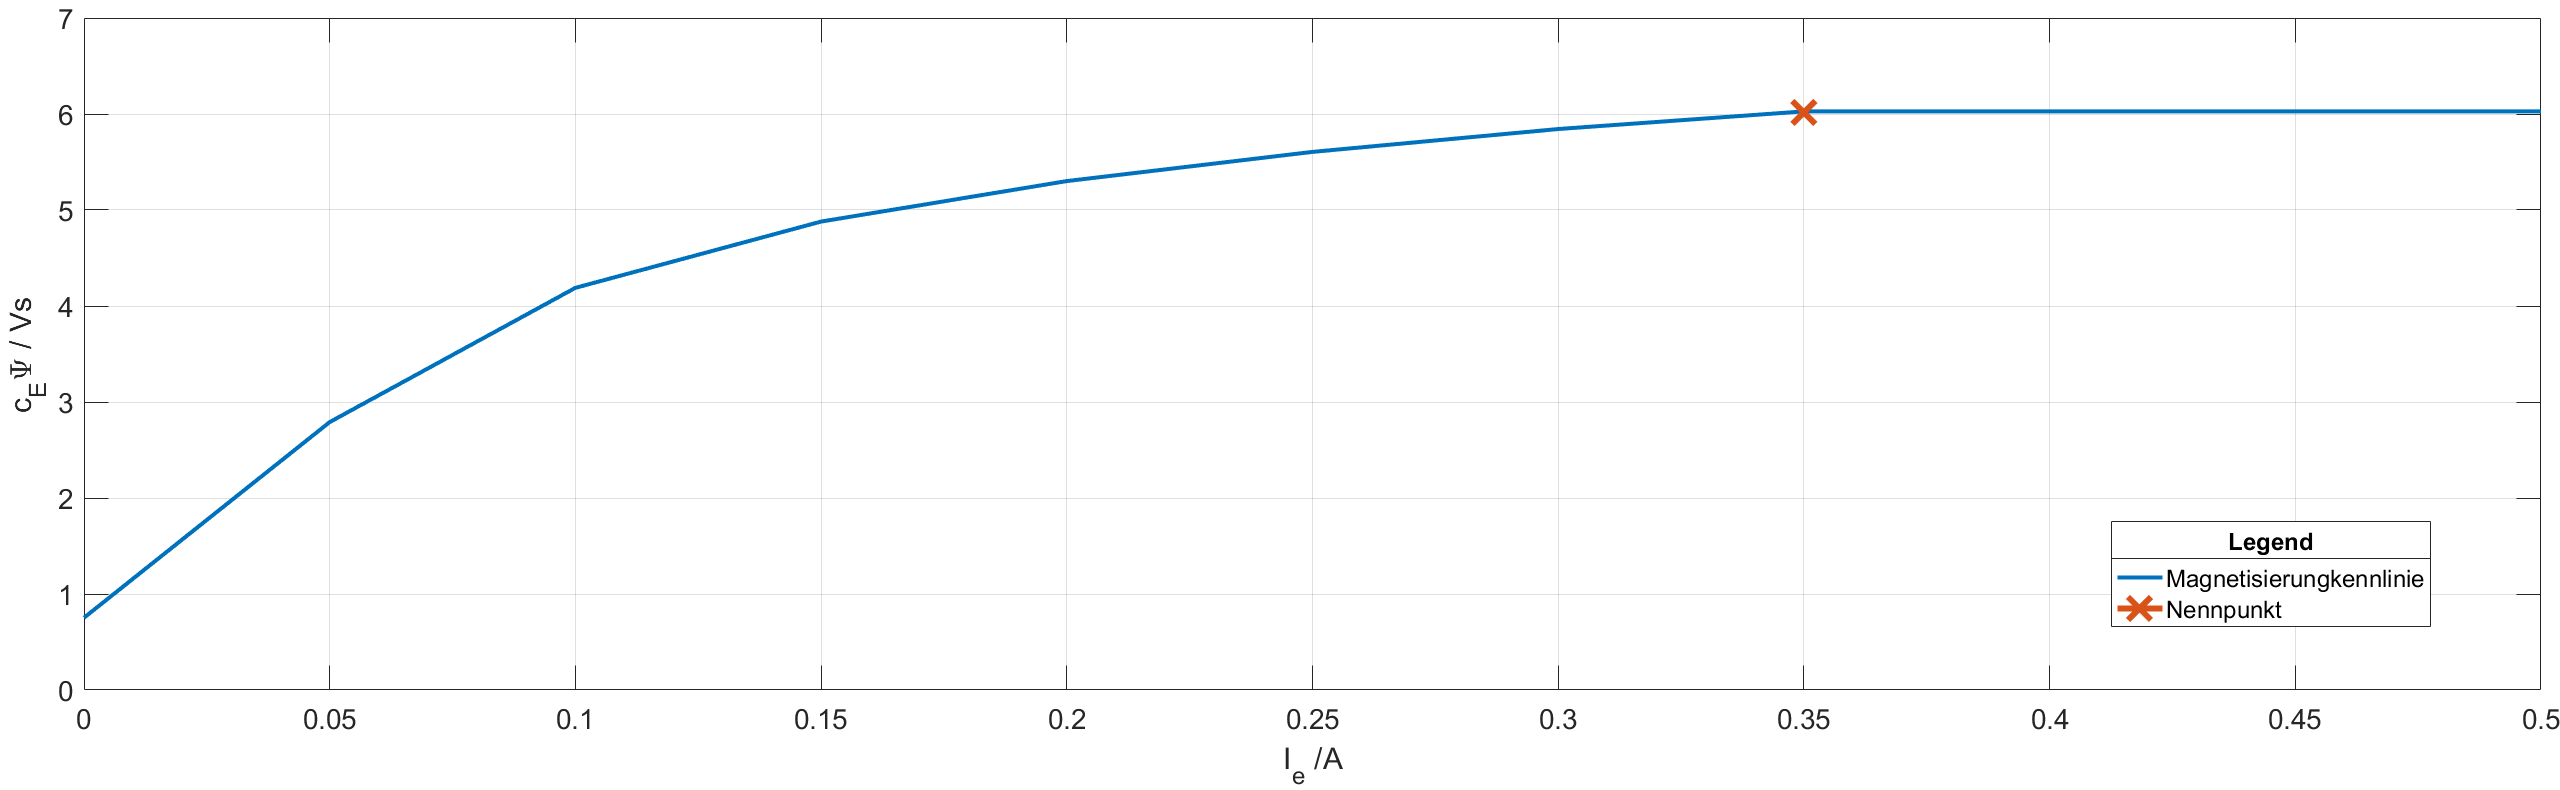
\includegraphics[width=1\textwidth]{./Bilder/magentisierungkennlinie_1}
\caption{Magnetisierungskennlinie}
\label{fig:magnet}
\end{figure}
%
\section{}\label{sec:aufg4_d}
%
Der Erregerstrom wird so eingestellt, dass eine Nennflussverkettung $\Psi_\text{N} = 6.016$Vs erreicht wird. Bei einem höheren Erregerstrom würde die Nennflussverkettung nicht, bzw. kaum steigen, weil der Eisenkern sich in Sättigung befindet. Bei niedrigeren Erregerströmen tritt bei schwankender Spannungsversorgung eine große Änderung des Flusses auf, da die Steigung der Magnetisierungskennlinie(siehe Abb. \ref{fig:magnet}) in diesem Bereich sehr hoch ist. Außerdem bei einer Absenkung des Feldes das Nennmoment erreicht werden (Feldschwächbereich).
%
\clearpage